\documentclass[10pt]{article}
\usepackage[utf8]{inputenc}
 
% 10pt permet de déterminer la taille de la fonte
\usepackage[utf8]{inputenc}

\usepackage{amssymb,amsmath,amsthm,amsfonts, bbm} 
% il s'agit de différents packages utilisés pour écrire des mathématiques en Latex

\usepackage{geometry}
\geometry{hmargin=2.3cm,vmargin=2.5cm}
% ce package permet de spécifier la taille des marges (h: horizontales; v: verticales)

\usepackage{array}
\usepackage{graphicx,graphics}
\usepackage{caption}
\usepackage{subcaption}
\usepackage{stmaryrd}
%\usepackage{minted}
\usepackage{dsfont}
\usepackage{titling}
\usepackage{pdfpages}
\usepackage{amsmath}
\usepackage{amsfonts}
\usepackage{epsfig}

\usepackage[section]{placeins}
% packages utilisés pour faire des tableaux, graphiques et mise en page

\usepackage{url}




\title{Compte-rendu Projet Python: \\ Création d'une intelligence artificielle pour le Tic Tac Toe $9\times9$ }
\author{Pierre Eustache - Laure-Hélène Genuyt }
\date{21 mai 2018}

\begin{document}

\maketitle

%\section{Objectifs du rapport}
 %Le rapport doit contenir les éléments suivants :

%\begin{itemize}
 %   \item instructions pour exécuter le programme
  %  \item
%description d’un point de design de code
%\item
%description d’un algorithme du programme et son coût
%\item
%description d’une difficulté qui vous a fait perdre beaucoup de temps (hors celles liées à votre apprentissage de la programmation)
%\item
%description d’une contribution originale
%\item
%description des résultats obtenus
%\item
%prolongements et applications envisageables

%\end{itemize}
\section{Introduction}
L'objectif de ce projet a été de créer une intelligence artificielle pour le jeu du Tic Tac Toe $9\times9$ (aussi appelé morpionception, ou Ultimate Tic Tac Toe). 
\paragraph{}


    \begin{enumerate}
    
\item \textbf{Règles du jeu}\\

Il s'agit d'un jeu de plateau, composé d'une grille de 3 cases par 3, dont chacune des cases contient elle-même une grille de 3 par 3. Dans la suite, on se référera à la "grande grille" et aux "petites grilles" pour distinguer ces deux niveaux de jeu.\\
L'objectif du jeu est de remporter 3 cases de la grande grille, en y apposant son symbole (une croix ou un cercle). Pour cela, les joueurs jouent au niveau des petites grilles, et cherchent à les remporter en alignant 3 de leurs symboles. Une fois la petite grille gagnée, on ne peut plus y jouer, et elle devient elle-même une case "croix" ou "cercle". \\
Le jeu présente cependant une subtilité qui le rend intéressant: chaque joueur doit jouer dans la case de la grande grille correspondant à la case de la petite grille où a joué l'autre joueur au tour précédent.


%\paragraph{}
%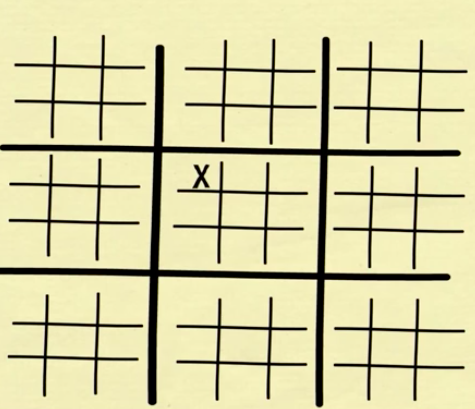
\includegraphics[width=0.25\textwidth]{tour1.png}
%\caption{Joueur A a joué dans la case en haut à gauche d'une petite grille} \\
%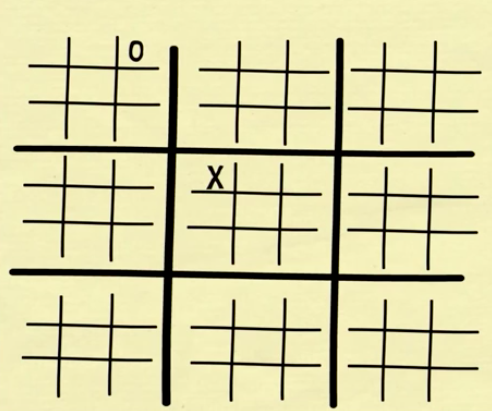
\includegraphics[width=0.25\textwidth]{tour2.png}
%\caption{Joueuer B doit donc jouer dans la case en haut à gauche de la grande grille} \\
%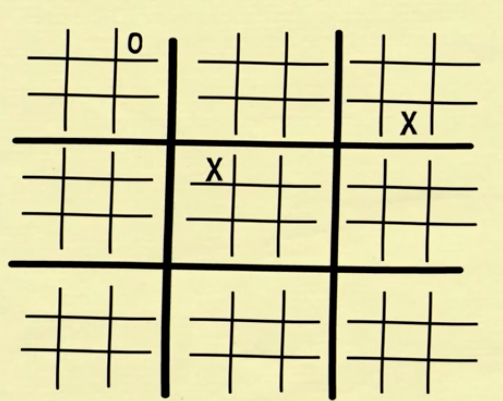
\includegraphics[width=0.25\textwidth]{tour3.png}
%\caption{Comme B a joué dans la case en haut à droite de sa petite grille, A doit jouer dans la case correspondante de la grande grille} \\
%\end{figure}


\begin{figure}
 \begin{minipage}[t]{0.25\linewidth}
  \centering\epsfig{figure = tour1.png,width=\linewidth}
  \caption{Dans cet exemple, A a joué dans la case en haut à gauche de sa petite grille.}
 \end{minipage} \hfill
 \begin{minipage}[t]{0.25\linewidth}
  \centering\epsfig{figure = tour2.png,width=\linewidth}
  \caption{Au tour suivant, B doit donc jouer dans la case en haut à gauche de la grande grille}
  \end{minipage} \hfill
 \begin{minipage}[t]{0.25\linewidth}
  \centering\epsfig{figure = tour3.png,width=\linewidth}
  \caption{Comme B a joué dans la case en haut à droite de sa petite grille, A doit ensuite jouer dans la case correspondantes de la grande grille (etc.)}
 \end{minipage}
\end{figure}


\paragraph{}
Lorsqu'un joueur renvoie l'autre dans une case de la grande grille déjà gagnée, celui-ci peut jouer où il le souhaite. \\

Le jeu se termine dès qu'un joueur a réussi à aligner 3 croix ou 3 cercles dans des cases de la grande grille. 


\paragraph{}
\begin{figure}[h!]
\centering
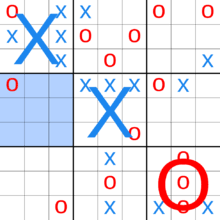
\includegraphics[width=0.5\textwidth]{exemple.png}
\caption{Exemple d'une partie de Tic Tac Toe $9\times9$}
\end{figure}

\item \textbf{Difficultés du jeu} \\

La création d'une intelligence artificielle pour ce jeu, en apparence relativement simple, pose quelques problèmes. 
En effet, contrairement au jeu du Tic Tac Toe classique, qui se termine par un match nul à moins d'une erreur d'inattention de la part d'un des joueurs, il est difficile de trouver une stratégie gagnante à ce jeu, et de bien en saisir tous les mécanismes.
\paragraph{}
De plus, la création d'une intelligence artificielle suppose de pouvoir évaluer chaque coup et de déterminer la valeur d'une position. Or, cela ne va pas de soi dans ce jeu, qui se joue à plusieurs niveaux: un coup doit-il être évalué à l'aune de ce qu'il apporte au joueur dans la petite grille où il est joué? \\
Ou faut-il davantage tenir compte de la case de la grande grille où il renvoie l'adversaire? 

\item \textbf{Méthode suivie}

\begin{itemize}
    \item Nous avons tout d'abord réfléchi à une manière optimale de coder une partie, et plus particulièrement l'état de la grille à un instant donné. Nous avons décidé de répresenter  la grande grille comme un tableau $3\times3$ de tableaux $3\times3$ (les petites grilles). Chacune des 81 cases est donc référencée grâce à un quadruple indice. \\
    \underline{Ex}: la position (1,1,3,3) fait référence à la petite case en bas à droite de la grande case en haut à gauche. \\ 
    Notre tableau est composé de 0, de 1 et de 2, où 0 représente une case vide, 1 une case contenant une croix, et 2 une case contenant un cercle. \\
    Nous avons ensuite créé un algorithme permettant de coder ce tableau en binaire, afin d'optimiser l'espace pris par une grille, mais cela ne nous as finalement pas servi par la suite.
   \paragraph{}
    \item Nous nous sommes ensuite servis du module \textit{tkinter} pour créer une interface graphique affichant l'état de la grille à un instant donné, à partir du tableau décrit précédemment. 
    \paragraph{}
    \item Afin de créer notre intelligence artificielle, nous avons essayé d'évaluer la valeur d'un coup grâce à une analyse heuristique. 
    En effet, contrairement à un jeu d'échecs, où la valeur d'un coup peut être assimilé à la valeur du pion qu'il permet de prendre, il est difficile de trouver une valeur objective d'un coup au Tic Tac Toe $9\times9$. Nous avons donc crée une fonction prenant en compte un certain nombre d'indicateurs qui nous semblaient entrer dans l'évaluation d'un coup, et attribuant à chacun une pondération - déterminée d'après notre avis subjectif et notre expérience du jeu dans un premier temps. \\
    Ces indicateurs sont: 
    \begin{itemize}
        \item la case que l'on compte jouer se trouve-t-elle dans un coin? 
        \item se trouve-t-elle au centre d'une case? 
        \item se trouve-t-elle au bord d'une case? 
        \item combien de symboles a-t-on dans la grille où on renvoie l'adversaire?
        \item combien l'adversaire possède-t-il de symboles dans la grille où on le renvoie?  
        \item la case où on renvoie l'adversaire est-elle déjà gagnée?  
        \item cette case est-elle vide? 
        \item ce coup renvoie-t-il l'adversaire dans une case qu'il peut gagner? 
        \item ce coup permet-il de remporter la case? 
        \item ce coup permet-il de gagner le jeu? 
    \end{itemize}
\paragraph{}
Ces indicateurs ont une pondération positive si on juge qu'ils sont en faveur du joueur, négative si on juge le contraire. \\
On part par exemple du principe qu'il est plus avantageux de jouer au centre que dans un coin, et plus avantageux de jouer dans un coin que de jouer au bord. \\
On considère également qu'il vaut renvoyer l'adversaire dans une case où il possède peu de symboles, et qu'il faut surtout éviter de l'envoyer dans une case déjà gagnée (ce qui lui permettrait de jouer n'importe où par la suite). 
\paragraph{}
\item Une fois cette heuristique créée, nous avons codé les règles du jeu (définition des coups possibles, enchaînement des actions, etc.), avant de créer une intelligence artificielle jouant aléatoirement selon ces règles (IA de type \textit{dummy} dans le code). 
\paragraph{}
\item Nous avons ensuite implémente un algorithme génétique dans le but d'améliorer nos pondérations, et de créer une intelligence artificielle jouant selon ces pondérations. \\
La performance de ces intelligences artificielles (de type \textit{heurist} dans le code) a été évaluée en fonction de leur taux de victoire et de défaite contre l'intelligence artificielle jouant aléatoirement. 
L'algorithme génétique se décompose en plusieurs étapes: 
\begin{itemize}
    \item créer un lot de joueurs, jouant selon des pondérations déterminées de façon subjective dans un premier temps. 
    \item faire jouer ces joueurs contre notre intelligence artificielle aléatoire, en enregistrant leurs scores. 
    \item une fois le tournoi terminé, trier les joueurs selon leur score, et en garder la meilleure moitié. 
    \item muter le reste des joueurs, en modifiant de manière aléatoire leurs pondérations. 
    \item avec ce nouveau lot de joueurs (meilleure moitié et joueurs mutés), recommencer à partir de la deuxième étape.   
\end{itemize}

\item Au bout de 30 générations, nous avons obtenu les résultats suivant sur 100 matchs: 

On voit donc que notre intelligence artificielle générée par cet algorithme génétique présente une très nette amélioration par rapport à notre intelligence artificielle aléatoire.
$$
\begin{tabular}{ |c|c|c| }
\hline
Type & Heuristique & Aléatoire\\
\hline
Victoires & 91 & 35 \\
\hline
Nuls & 5 & 30 \\
\hline
 Défaites  & 4 & 35 \\
 \hline
\end{tabular}
$$
\paragraph{}
\item Cette intelligence artificielle heuristique présente cependant une faiblesse majeure, qui est qu'elle n'a aucune profondeur dans son évaluation des coups: elle joue simplement selon des pondérations permettant d'évaluer la valeur du coup qu'elle va jouer \\
Nous avons donc implémenté un algorithme minimax, permettant à l'IA de voir à une profondeur de 3 coups. \\
Cet algorithme, que l'on peut représenter sous forme d'un arbre, examine toutes les évolutions possibles du jeu à partir de la configuration actuelle,et attribue à chacune de ces feuilles une valeur (selon les pondérations de la meilleure intelligence artificielle générée par l'algorithme génétique). \\
On considère que l'adversaire (qui joue au coup d'après), va choisir le coup qui l'amène à la situation la plus bénéfique pour lui, et donc la plus néfaste pour nous. \\
La valeur d'un nœud de l'adversaire correspond donc au minimum des feuilles évaluées précédemment. La valeur de chacun de nos coups possibles va donc être le maximum des valeurs des nœuds de l'adversaire, et on va jouer le coup possédant la plus haute valeur (il s'agit donc du coup qui nous permettra d'atteindre la situation de jeu la plus optimale pour nous dans 3 coups, en sachant que l'adversaire choisira toujours le coup qui lui est le plus avantageux).

\paragraph{}
\begin{figure}[h!]
\centering
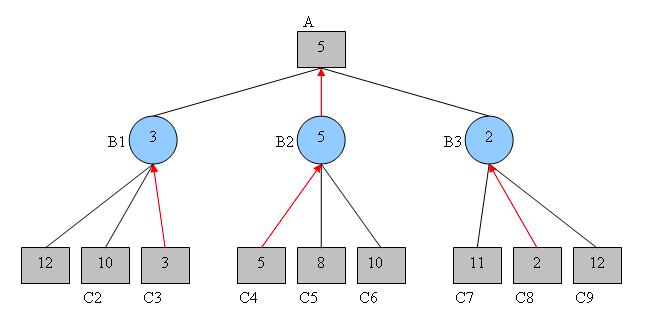
\includegraphics[width=0.7\textwidth]{minimax.png}
\caption{ }{Exemple d'arbre minimax (les carrés représentent ici les nœuds joueurs et les ronds les noeuds opposants)}
\end{figure}


Cet algorithme permet à l'intelligence artificielle de gagner en performance. \\
Contre l'intelligence artificielle aléatoire, on a en effet observé, sur 200 matchs: 
$$
\begin{tabular}{ |c|c|c|c| }
\hline
Type & Minimax & Heuristique & Aléatoire\\
\hline
Victoires & 187 & 181 & 70 \\
\hline
Nuls & 10 & 10 & 60 \\
\hline
 Défaites & 3 & 8 & 70 \\
 \hline
\end{tabular}
$$

\paragraph{}

\section{Exécution du programme}
Le programme est implémenté prêt à jouer contre l'utilisateur. En effet, l'IA par défaut est déjà correctement paramétrée en ayant en mémoire l'une des plus prometteuses pondérations trouvée durant notre algorithme génétique.
\par Cependant, le programme permet à l'utilisateur de manipuler à loisir les différentes génération et d'ainsi pouvoir lui-même voir se dérouler des parties entre différentes IA de son choix.
\par \underline{usage:}
\begin{itemize}
\item \textit{Player(pond = [float], typ=str)}\qquad avec \emph{pond} les pondérations de l'IA, et \emph{typ} pouvant prendre les valeurs :
\begin{itemize}\item \emph{"dummy"} $\rightarrow$ aléatoire
\item \emph{"heuri"} $\rightarrow$ simple heuristique
\item \emph{"mini"} $\rightarrow$ heuristique + minimax
\end{itemize}
\item \textit{Game(p1=Player(), p2=Player())} \qquad avec \emph{p1, p2} respectivement le premier et le second joueur à jouer.
\item \textit{Game.hist()} \qquad affiche un historique de la partie.
\end{itemize}
Le programme a également été optimisé pour rendre automatique l'algorithme génétique, si l'utilisateur désire tenter de développer sa propre colonie.

\begin{itemize}
\item $training(nb=int, gen= int, nb\_games=int)=list[Player]$ \par Génère une couvée de \emph{nb} joueurs, sur \emph{gen} générations, en leur faisant vivre \emph{nb\_ games} pour les départager.
\item $mut\_range = 6$ \qquad Détermine l'ampleur de la mutation à chaque génération
\item $random\_range = 10$ \qquad Détermine à quelle distance de $0$ se trouvent les initialisations de l'algorithme génétique.
\end{itemize}



\section{Améliorations et perspectives}
Le programme peut encore être amélioré.
\subsection{Interface graphique}
L'interface graphique actuelle est très sommaire car elle n'a été développée que dans des perspectives de test et de debug. Dans cette optique, il serait possible d'implémenter une interface plus complexe qui permettrait de commander les opérations implémentées facilement et lancer des parties contre différentes IA, de difficulté croissantes.
\par Il serait également possible de faire l'exact exemple et d'incorporer un éditeur d'IA qui permettrait de défier ses amis en développant une IA battant la leur, à la manière de LeakWars\footnote{\url{https://leekwars.com/}}.

\subsection{Intelligence artificielle}
L'étape suivante dans la quête d'une IA serait d'adopter le paradigme du réseau de neurone afin de remplacer l'heuristique. En effet, il serait intéressant d'entraîner un réseau de neurone qui noterait a position d'arrivée et permettrait de choisir un coup de manière à maximiser sa valeur d'arrivée.
\par Cela nécessiterait de passer de la méthode actuelle de notation qui se fait en fonction du coup proposé, et de la situation actuelle, à une notation d'une grille seule.

\subsection{Applications}
Il est extrêmement difficile de résoudre entièrement le morpionception. Le nombre de grilles est bien trop élevé sans avoir recours à des techniques de mémoïsation, un stockage particulier, et une RAM très importante afin de générer l'arbre de jeu. Cependant, en appliquant des techniques de deep learning en mettant en place une IA assez efficace, prouver que cette IA gagne toujours serait la démonstration d'une stratégie - bien qu'éventuellement peu régulière - gagnante.
\par Il est également possible de transformer le tout en jeu.

\end{itemize}
\end{enumerate}
\end{document}
